\subsection{Cross Sections as a function of the neutrino-muon opening angle}
%Results in $\theta_{\mu}$ }

The differential cross section as a function of $\theta_{\mu}$ for interactions on the CH, C, H$_{2}$O, Fe, and Pb targets, respectively, are shown in Fig.~\ref{figure:xsec_muon_theta}. $\theta_{\mu}$ is the angle of the muon with respect to the neutrino beam direction.  The uncertainties broken down by source for both the absolute cross sections and the cross section ratios as a function of $\theta_\mu$ can be found in Fig.~\ref{fig:xsec_err_muon_theta}.  
%The data are represented by the black dots with error bars.  The expectation from the simulation (MnvGENIE) is given by the histograms and is broken down by the interaction process.  

% tki_muon_theta xsecs
\begin{figure}[h] 
	\centering
  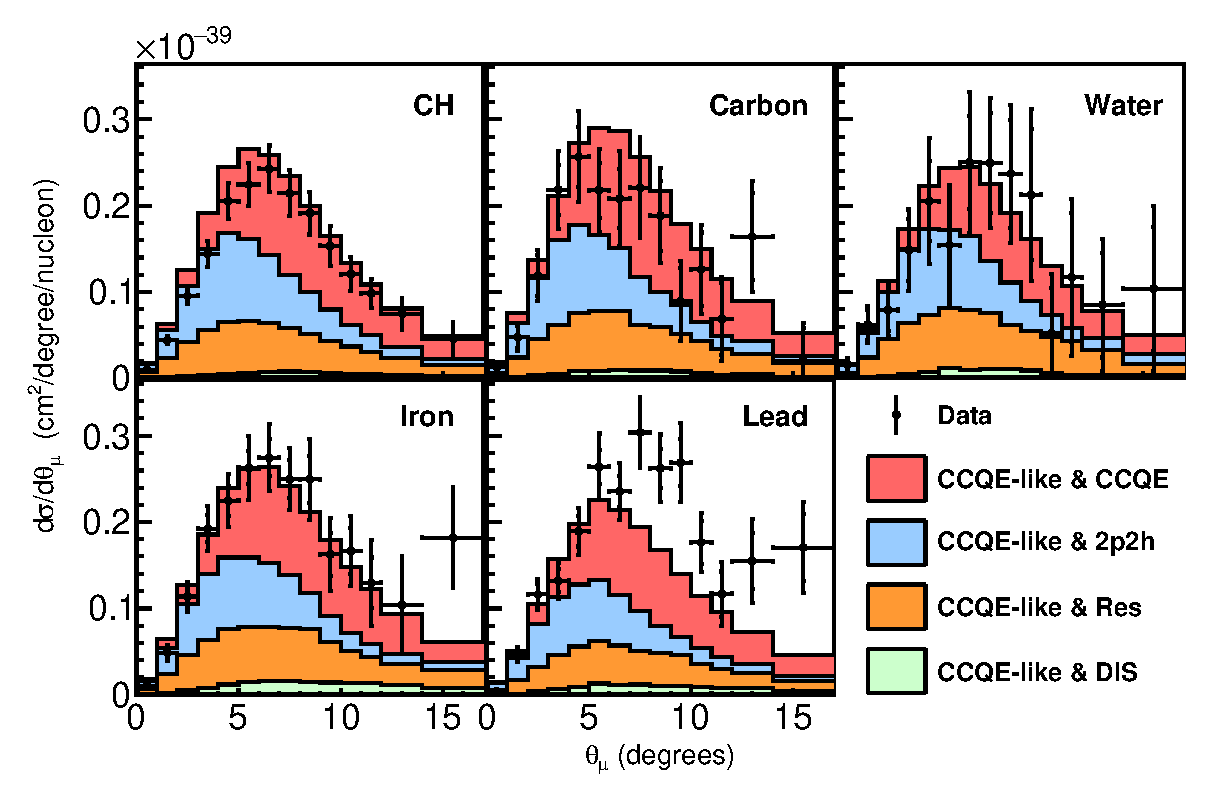
\includegraphics[width=\linewidth]{Figures/xsec_five_square/muon_theta.eps}
	\caption{The differential cross section as a function of $\theta_\mu$ for CH, C, H$_{2}$O, Fe, and Pb targets, along with the predictions for the different quasielastic-like signal processes.}
	\label{figure:xsec_muon_theta}
\end{figure}


%Here it appears that the data tend to be slightly broader in $\theta_{\mu}$ than MnvGENIE.  Although the uncertainties are large for the data taken on the C and H$_{2}$O targets, this trend seems to cut across all the nuclear targets.  

In scintillator, the MINERvA tune has more cross section at lower $\theta_{\mu}$ than is seen in the data.  This trend is not present for the data taken on C, as might be expected for consistency with scintillator, although the uncertainties are larger for this data.
There is significantly more cross section in the tail at higher $\theta_{\mu}$ in the data than in the MINERvA tune for data taken on the Pb target.

The differential cross section as a function of $\theta_{\mu}$ for the different targets as compared to a range of models is given in Fig.~\ref{fig:models_muon_theta}. 
Most of the models investigated have an expectation shifted to slightly smaller angle than that seen in the data.  NEUT exhibits a higher cross section than the data in general.  This is also seen for the hN versions of GENIE for the Pb target.  The \chisq\ between the cross sections and the models can be found in Table~\ref{tab:muontheta}.

% comparisons to generators muon_theta
\begin{figure}[h]
    \centering
    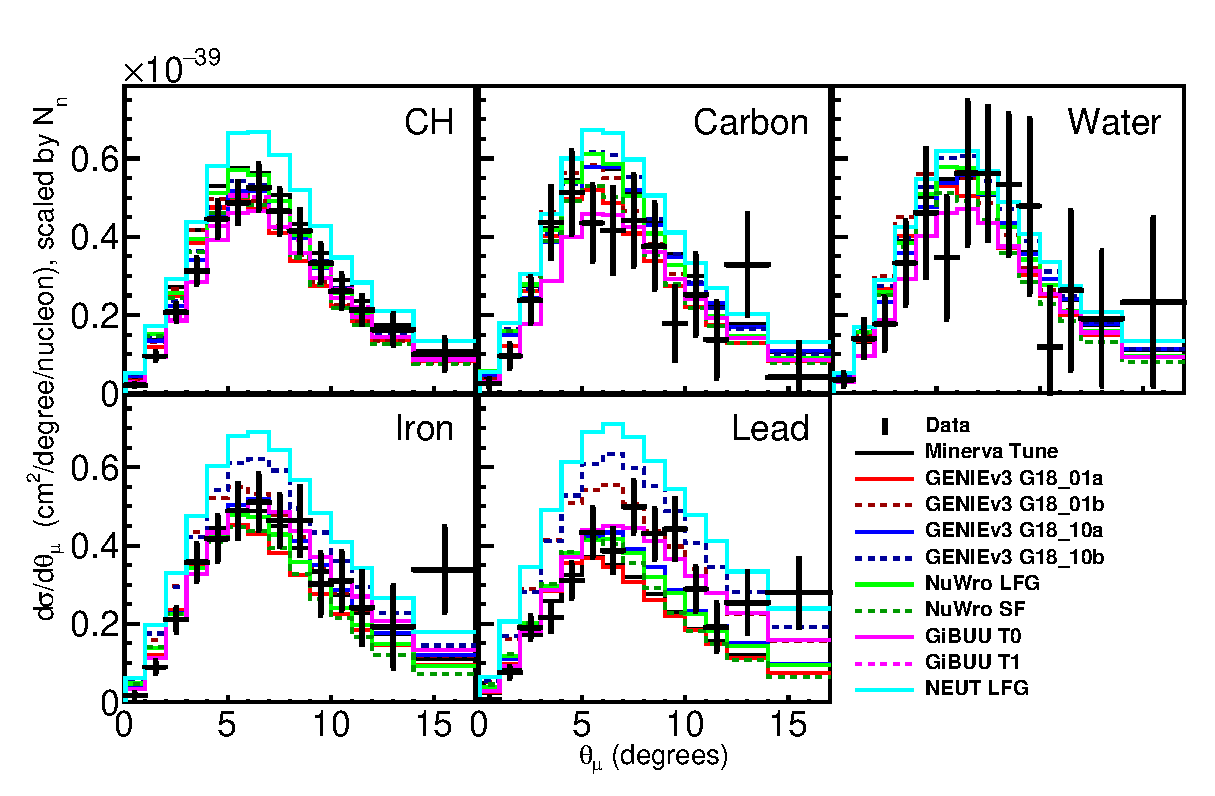
\includegraphics[width=.8\linewidth]{Figures/gencompare/muon_theta_5square.eps}
    \caption{Cross section measurements and predictions as a function of $\theta_\mu$ for different targets and for a selection of different generator and model choices.}
    \label{fig:models_muon_theta}
\end{figure}


The ratio of the differential cross section as a function of  $\theta_{\mu}$ for each nuclear target (C, H$_{2}$O, Fe, Pb) to that for scintillator is shown in 
Fig.~\ref{Figure:Gencompare_mutheta_ratio}.  
The angle seems well modeled and the scaling with the number of neutrons works well up through the Fe data.  For the data taken on Pb, the data ratio tends to peak at a larger angle than what is seen in the models.
The \chisq\ between the cross section ratios and the models can be found in Table~\ref{tab:muontheta}.
\begin{figure}
    \centering
                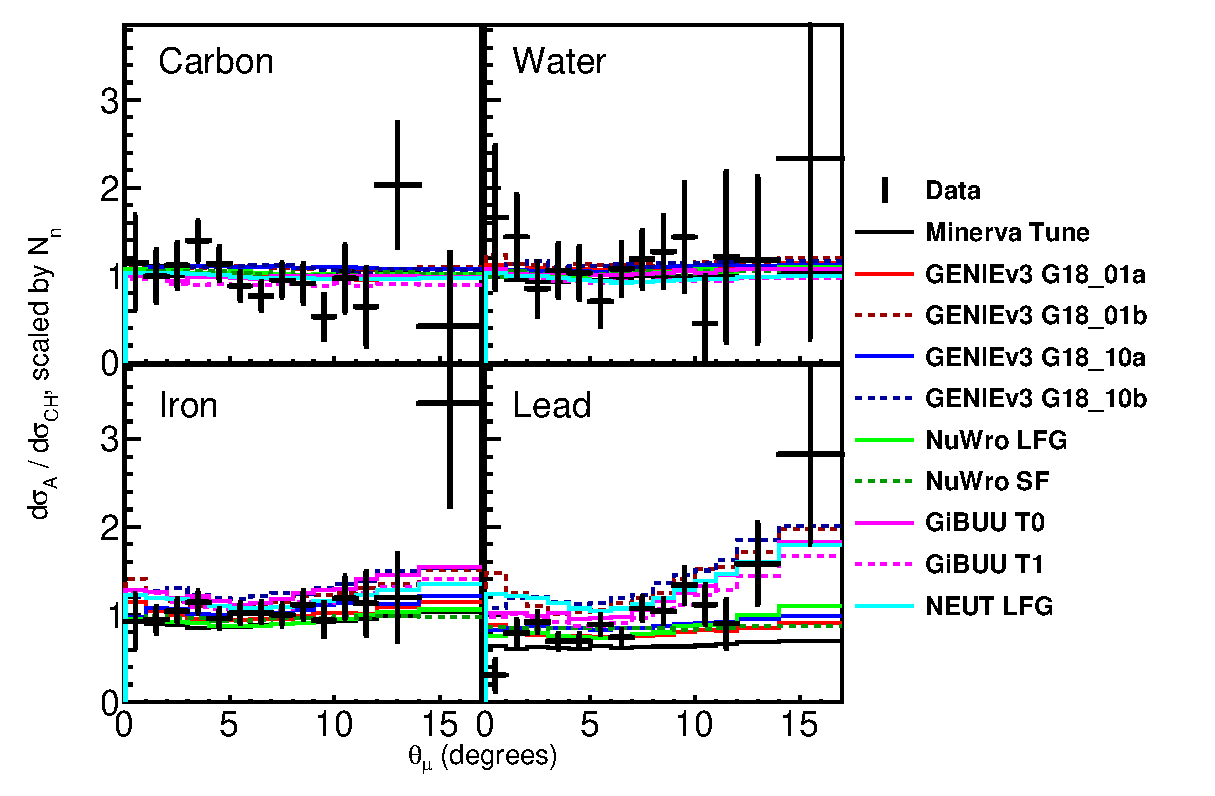
\includegraphics[width=\linewidth]{Figures/gencompare/muon_theta_4square.eps}
    \caption{$\theta_\mu$ cross-section ratio generator comparison for multiple targets.  Changes to the FSI model (GENIE ``a'' to ``b'') in GENIE change the cross section ratio more than changes to the 2p2h model (GiBUU T0 to GiBUU T1) or changes to the initial state (GENIE 1 to GENIE 10) or (NuWro LFG to NuWro SF).  The changes to the ratio are most significant at high muon angle.}
        \label{Figure:Gencompare_mutheta_ratio}
\end{figure}
